% !TEX root = paper.tex
\section{Introduction}

The volume of traffic on our roads has been growing steadily for over 25 years, both in terms of the number of vehicles on the road -- increasing by 40.6\% in the UK~\cite{noVehiocles} -- and the distances covered -- 325.5 billion miles driven in the UK in the year ending September 2017 which is up nearly 30\% in the last 25 years~\cite{distance}. This is placing ever more burden on the road infrastructure along with those who police and manage it. In order to better understand how we can deal with this increase in demand we need to better understand how the road network is being used. By understanding road usage we can better deal with congestion, handle traffic incidents, plan road modifications and deal with illegal acts on the roads.

In a utopian model we would have full disclosure of all journeys made by all vehicles on the road infrastructure. However, this has numerous ethical and technical issues. From an ethical standpoint should we be allowed to know where all vehicles are at any given point in time. From a technical point of view, although every vehicle could be fitted with a GPS tracker -- costly in its own right -- there would still exist the issue of how we would collect and stream all of this data for future processing. Alternatively one can view the problem the other way around and rather than tracking individual vehicles look at collecting information by observing vehicles passing points within the road networks. A prime example of this approach are Automatic Number-plate Recognition (ANPR) cameras. These cameras are a combination of digital camera coupled with Artificial Intelligence to identify number-plates within the image and convert these into strings of characters. ANPR cameras are normally fixed in location\footnote{Although cameras can be in a vehicle and moved from location to location.} able to view all vehicles passing that location.

For ANPR the problem now becomes that of recovering as much information about vehicle's journey as possible from the limited number of observations. ANPR cameras are normally located on major roads and interchanges, however, this only covers a tiny fraction of the road network. We can, though, estimate routes between cameras by understanding the distances between cameras and the most ``sensible'' routes between them. This allows us, given a set of ANPR sightings of the same vehicle, to produce a ``most likely'' route for that journey. It should be noted that we cannot determine the actual start and end of the journey as these will happen in areas not covered by ANPR. It should also be noted that for ethical reasons it is not normal to obtain actual number-plates, but rather the hash of these. Though, for most situations this will suffice.

Once we have a set of sightings of a vehicle using ANPR, we now need to convert these into actual journeys. The first requirement is to identify individual journeys. Although this can't be done with certainty we can apply general rules to distinguish one journey from the next. For example if two sightings are made from ANPR cameras which are connectable by a ``sensible'' route\footnote{Here ``sensible'' implies that a route between cameras A and B would not need to go through a third camera C.} in a time interval which is ``sensible'' then these can be determined to be part of the same journey. However, if the timings between two sightings is significantly longer than what would be expected then this would imply that the vehicle stopped between these two cameras and that the later sighting is part of a new journey.

The process of journey identification needs to be performed on dirty data which contains numerous impurities which need to be handled. These include:

\begin{itemize}
	\item {\bf Number-plate miss-reads:} Although ANPR cameras have accuracies of around {\color{red}99\%}, miss-reads are possible. This can lead to sightings being missed or vehicles being wrongly sighted in locations.
	\item {\bf Timing errors:} The time-stamps of sightings could be erroneous. The minor side of this is implausible journey times, though, more seriously, this can lead to reordering the set of cameras on a particular journey.
	\item {\bf Clones number-plates:} For various reasons a number-plate may be cloned and used on a different vehicle. This can lead to impossible journeys and journeys that the real vehicle did not make.
\end{itemize}

Once journeys have been identified from the sightings we can then progress by using these journeys to identify higher-order issues within the road network. In this paper we demonstrate how we can use this journey information in order to identify the most likely class each vehicle is a member of. By clustering over such characteristics as how many journeys are made each day, average length of journeys, the number of different ANPR cameras seen in a day and the times when journeys are made we can cluster vehicles into buses, taxis, commuters and delivery vehicles.

The rest of this paper is presented as follows. In Section \ref{s.related} we discuss related work. Section \ref{s.ncl} we presents the ANPR data for the Newcastle area. Our process for identifying individual journeys is presented in Section \ref{s.trips} while Section \ref{s.classification} presents our classification approach. We present results in Section \ref{s.results} before offering conclusions and future directions in Section \ref{s.conclusions}.

\section{Related Work}
\label{s.related}

\begin{figure}[t]
\centering
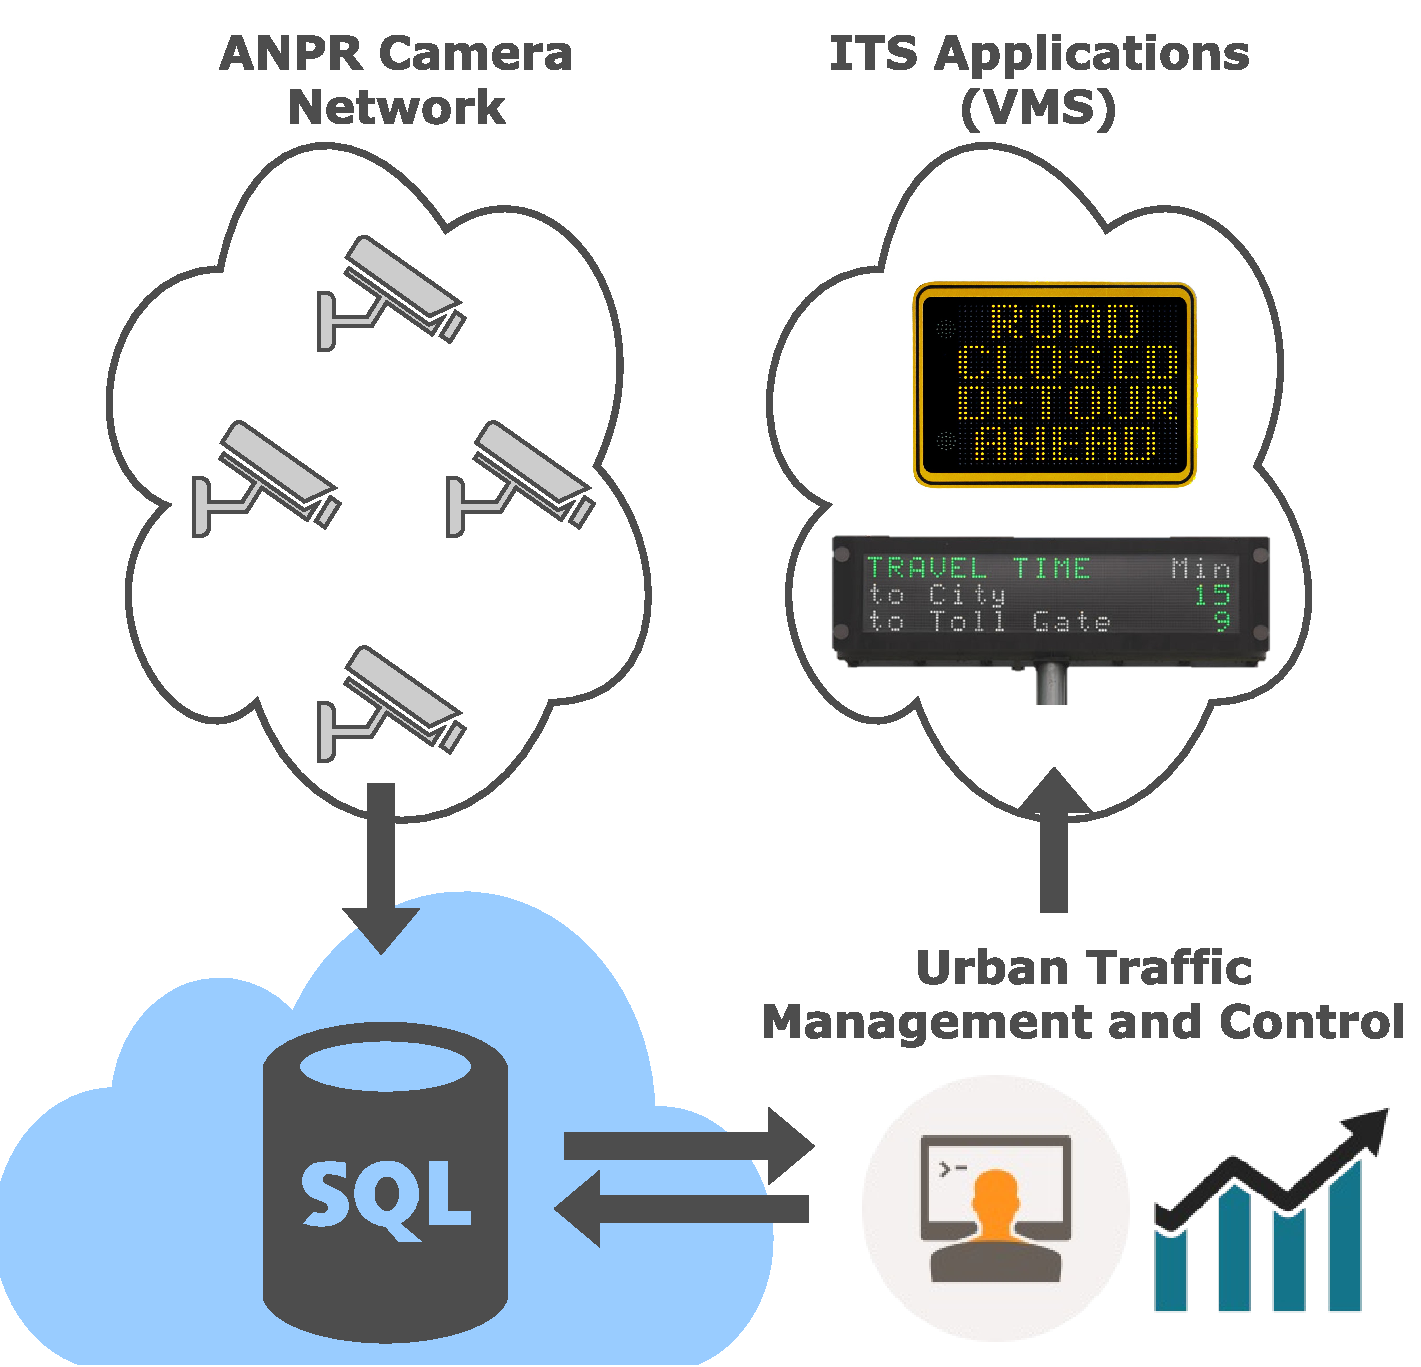
\includegraphics[width=.95\linewidth]{ANPR-overview.pdf}
\caption{Automatic number plate recognition system overview.}
\label{fig:anpr-overview}
\end{figure}

The main use of ANPR data for the UTMC is estimating average journey times for selected or sensitive links in the road network. Furthermore, several authors have extensively researched how to use number-plate data as an extension to link counts for estimating origin-destination matrices and link flows~\cite{Castillo2010, Castillo2008, Hazelton2012}. However, very few works have focused on analysing individual or collective travel patterns from number-plate data, particularly across extended periods of time. Moreover, there is no consistent conceptual and analytical framework for transforming number plate data into a historical sequence of trips for each vehicle. Finally, we believe that trip data, properly identified from number-plate data, has the potential to unlock a number of new applications for urban traffic control and law enforcement. Thus, in section~\ref{s.trips} we present a conceptual methodology for grouping multiple camera observations of the same vehicle into one or several trips of that vehicle.

Determining the distribution of travel modes is one of the fundamental steps in the four-stage model: an essential traffic modelling methodology for transportation planning~\cite{FourStepModel}. Previous works have used trip information derived from different sources of data to identify travel mode or purpose of trip. More notably, survey data, floating car data and mobile phone data have been used~\cite{ODMobileData, ClusteringGPS}.  Although number plate data has been used in~\cite{Clustering}, to identify different categories of trips, the authors do not differentiate between private or public travel modes and focus instead on categorising trips by time of occurrence. Hence, in section~\ref{s.classification} we apply the \emph{k-means} clustering algorithm to derived trip data and based on the results, we discuss the limitations of proposed methods and that of ANPR data.

% However, Furthermore, ANPR cameras can either be fixed or

% {\color{red}Uses of trip data for understanding travel demands / traffic prediction
%
% Studies about best placement of cameras
%
% Number plate data is not as popular, for urban traffic monitoring and prediction, as other sources of data, namely GPS traces or floating vehicle data.
% Previous works trips from GPS traces, .
%
% %Therefore, number plate scans provide additional trip information, besides simple link counts, that has
%
%  %estimating travel demands and traffic states. extended traditional methods of  travel demands
%
%
% Although significant research has gone into identifying trips from GPS traces, to the best of our knowledge, little research has gone into doing so with number plate data. Therefore, the contributions of this paper are twofold:

% \begin{enumerate}
%   \item
% \end{itemize}
